\documentclass[12pt,conference]{IEEEtran}
\usepackage{url}
\usepackage{graphicx}
\usepackage[norule]{footmisc}
\graphicspath{ {./images/} }
\usepackage{float}
\floatstyle{boxed} 
\restylefloat{figure}
\usepackage{physics}

% footer style
\makeatletter
\def\footnoterule{\kern-3\p@
  \hrule \@width 2in \kern 2.6\p@} % the \hrule is .4pt high
\makeatother

% paragraph indentation
\setlength{\parindent}{2.5em}
\setlength{\parskip}{1em}

% disable word break
\tolerance=1
\emergencystretch=\maxdimen
\hyphenpenalty=10000
\hbadness=10000




\begin{document}

\title{Quantum Annealing and Experience with D-Wave Systems}
% \IEEEspecialpapernotice{(Invited Paper)}


\author{\IEEEauthorblockN{Dhruvil Gandhi}
\IEEEauthorblockA{Seidenberg School of Computer \\Science and Information Systems,\\
Pace University\\
Email: dgandhi@pace.edu}
\and
\IEEEauthorblockN{Akshay More}
\IEEEauthorblockA{Seidenberg School of Computer \\Science and Information Systems,\\
Pace University\\
Email: amore@pace.edu}}


\maketitle

\begin{abstract}
\footnote  {about IBM supported class}This survey paper is an exploratory paper for D-Wave systems and using their Ocean Software. D-Wave systems offer adiabatic quantum computing through quantum annealing, we plan to use this to evaluate their examples. --tobechanged
\end{abstract}

\begin{IEEEkeywords}
Quantum Computer, Quantum Annealing, Optimization Algos, D-Wave, Hamiltonian
\end{IEEEkeywords}









\section{Introduction}
Quantum Computing has evolved significantly this decade. With a lot of services, infrastructures and tool kits commercially available to the public, there has been a great advancement in the field of quantum computing. A quantum computer takes advantage of the  propoery of qubit to exist in more than one state at any time. Compared to classical comouting, based on binary bits 0 and 1, quantum computers are based on 'qubits', which can store a lot more information than classical bit due to its propoery to be able to exist in more than one state. 

Various companies have made their quantum computers available to the public, IBM with Q-Experience, D-Wave Systems with D-Wave 2000Q, Regitti, Alibaba, Microsoft, Google, to name a few. All this quantum computers works on different approaches of quantum computing.

IBM created first universal quantum computer. D-Wave created adiabiatic quantum computer. There are a lot of resources available to learn and experiment with these systems. Through the paper, we briefly understand what a universal quantum computer is, different types of quntum computing, advantages and disadvantages. We explore D-Wave Quantum Computer, the principle it works on, implement optimization algorithm and show the results. 


\section{Background}

\subsection{Universal Quantum Computer}

\floatstyle{plain}
\restylefloat{figure}
\begin{figure}[h]
  \centering
  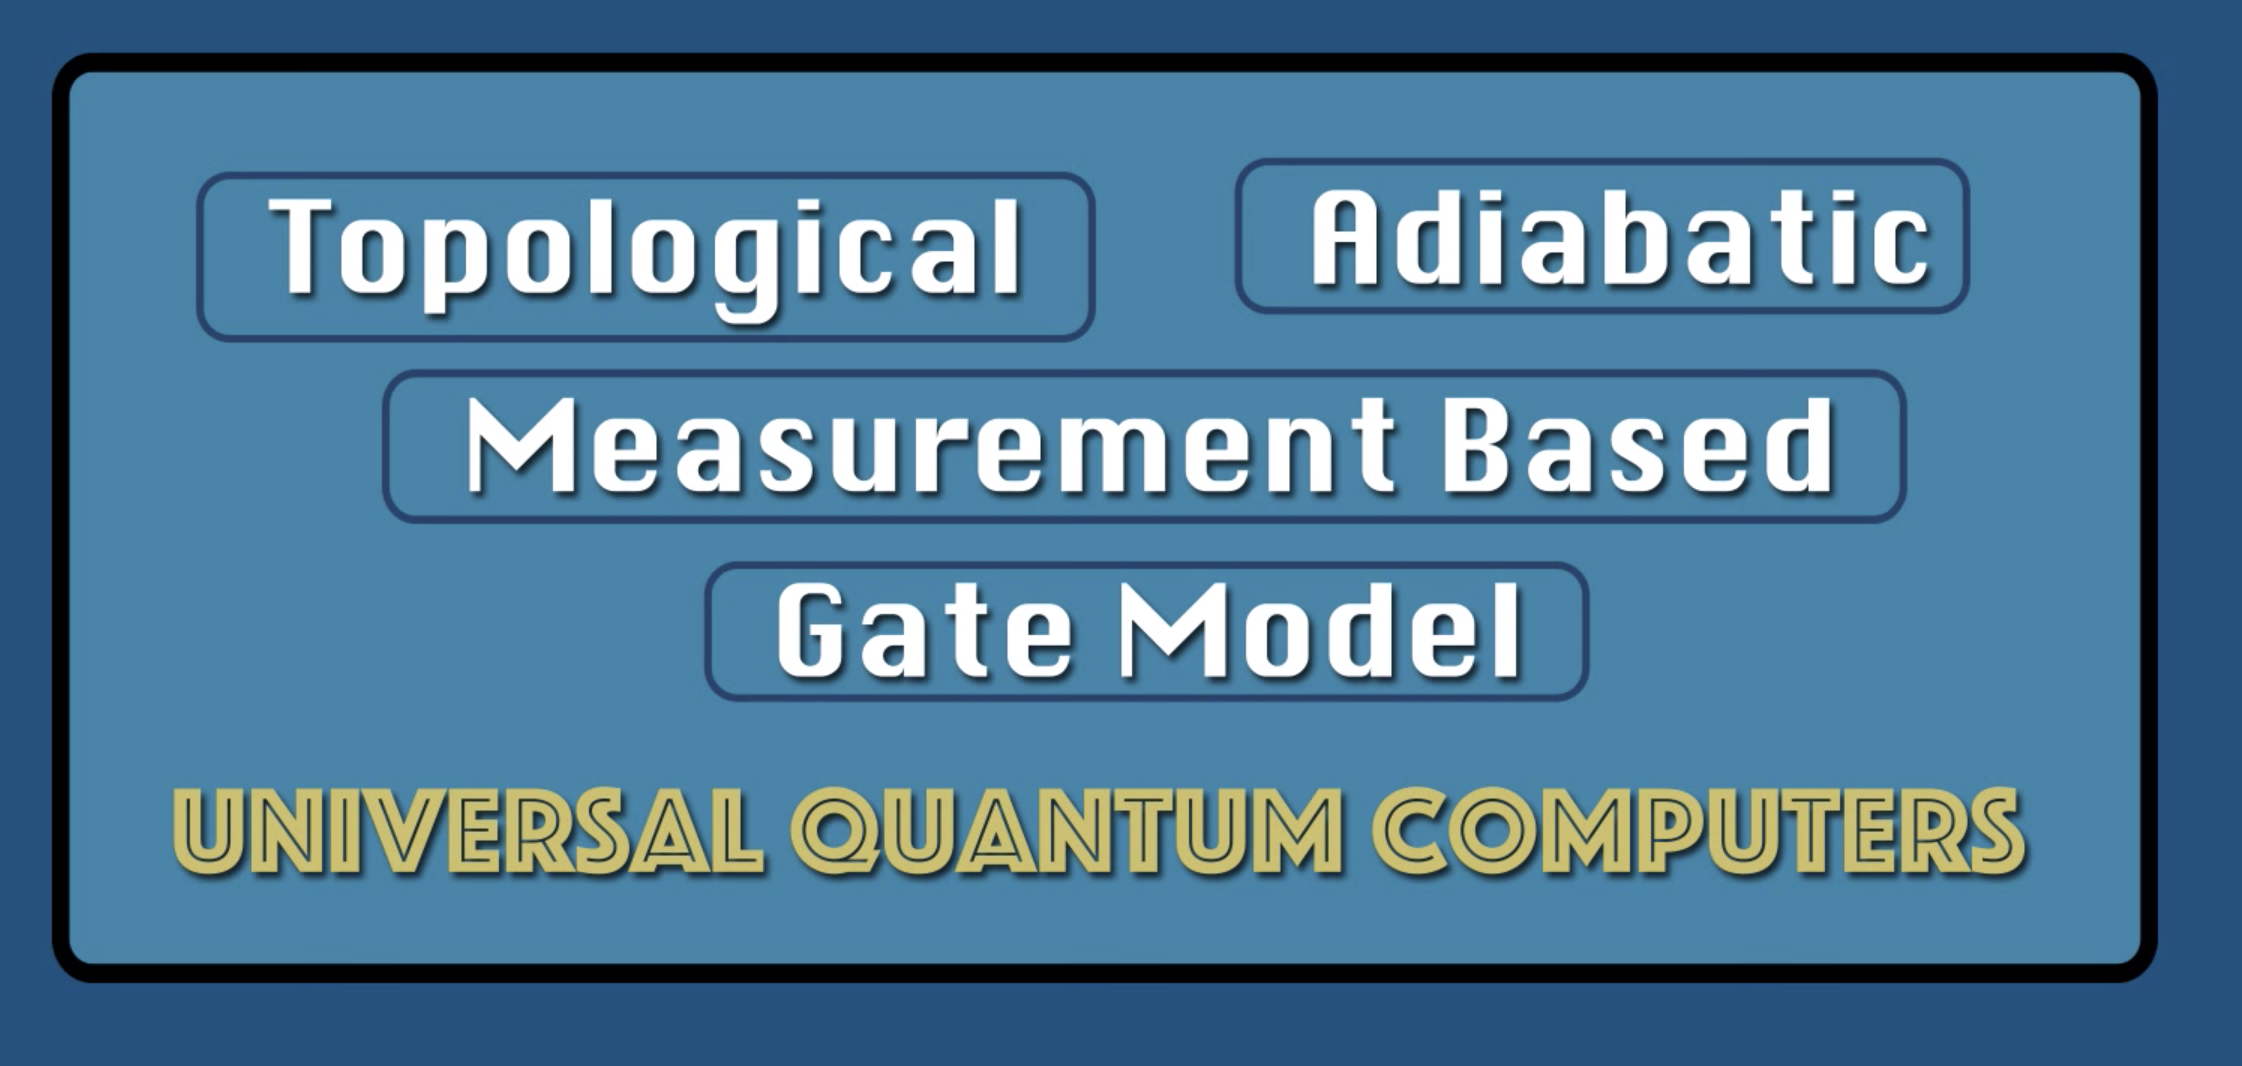
\includegraphics[width=8cm]{uqc.png}
  \caption{Universal Quantum Computers}
  \label{fig:UniversalQC}
\end{figure}

The first quantum computer was built using gate model approach where we control and manipulate state of the Quantumn bits or qbits to do operations and run algorithms. The Universal Quantum Computer is a one where we gate model approach is able to map to other forms of quantum computing in polynomial time and polynomial resources. Various approaches of qantum computing are:
\begin{itemize}
  \item Circuit Based Quantum Computing
  \item Adiabiatic Quantum Commputing
  \item Topological Quantum Computing
  \item Measurement Based Quantum Computing
\end{itemize}

\floatstyle{plain}
\restylefloat{figure}
\begin{figure}[h]
  \centering
  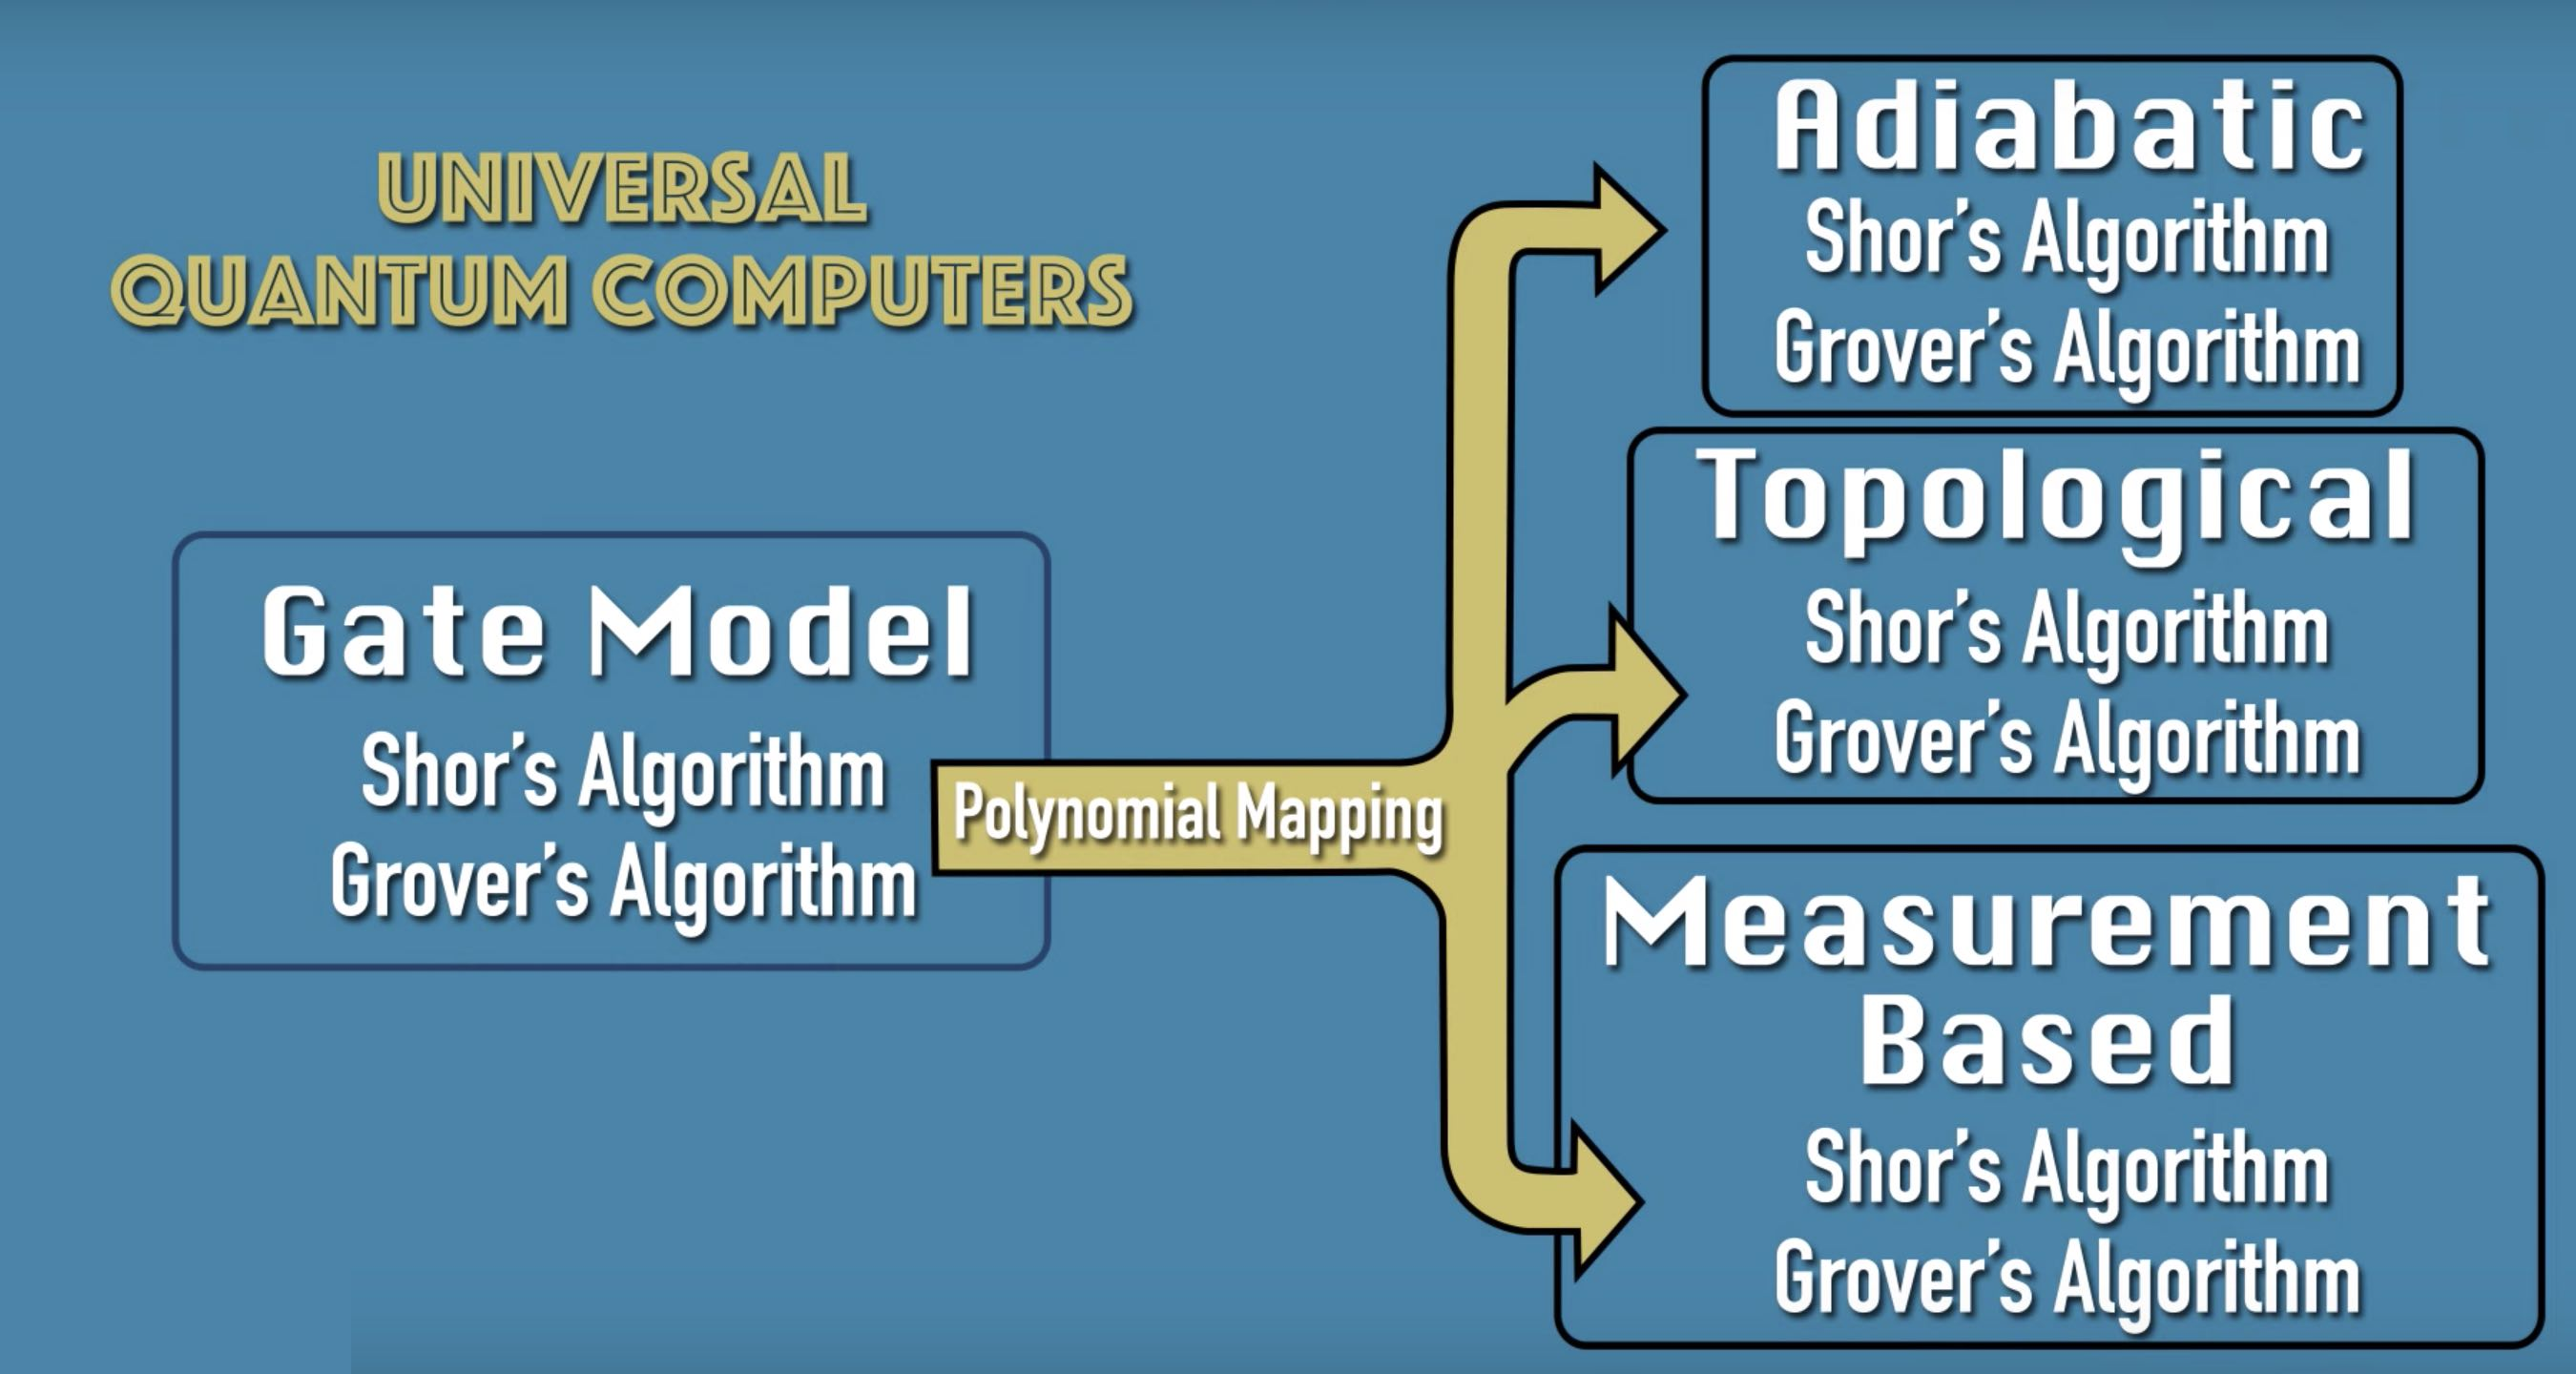
\includegraphics[width=8cm]{uqc_mapping.jpg}
  \caption{Polynomial mapping}
  \label{fig:PolynomicalUQC}
\end{figure}

To be a universal quantum computer, a quantum computer must be able to operate all the above approaches of quantum computing.







\subsubsection{Gates based}
In gate based quantum computing, the gates are built on the principle of qubits: \emph{superposition} and \emph{entanglement}.

\paragraph{Superposition}
Qubit can exist in both 0 and 1 state. It can be represented by the equation:
\begin{equation*}
  \ket {\psi} = a_0 \ket{0} + a_1 \ket{1}
\end{equation*} 
where a\textsubscript{0} and a\textsubscript{1} are configuration that specifies all the possibilities of state being in 0 and 1.

\paragraph{Entanglement}
In quantum computing, in a multi-particle system, entanglement is property of qubits where the state of one qubit cannot be described independently. To express the state of system with two Particles A and B, the quantum state can be described as tensor product of two state space described by the equation:
$\ket {\Phi} = \ket{A} \otimes \ket{B}$
or, it can be also written as
$\ket {\Phi} = \ket{AB}$


\subsubsection{Adiabiatic Quantum Computer}
Adiabatic quantum computing is based on Hamiltonian framework for quantum mechanics. Quantum systems evolves by unitary operators. We find the initial easily implementable Hamiltonian H\textsubscript{0}, find a path H\textsubscript{t} and find the final Hamiltonian H\textsubscript{1} keeping the system in ground state which depends on eigen gap. The basic principle of the adiabatic quantum computing is: as long as the path is traversed slowly from H\textsubscript{0} to H\textsubscript{1}, the system remains in ground state and the required solution is obtained. If traversed faster, the system jumps state and it results in error. 

\paragraph{Hamiltonian Formula} 
The Hamiltonian formula can be simplified as follows:
\begin{multline*}
  \mathcal{H}_s(s) = \frac{-1}{2} \sum_i \Delta (s) \sigma_i^x  \\ + \epsilon(s) ( - \sum_i h_i \sigma_i^z + \sum_{i<j} J_{ij}  \sigma_i^z \sigma_j^z)
\end{multline*}
which can be broken down as:
\begin{itemize}
  \item[$-$] $\mathcal{H}_s(s)$ is the required Hamiltonian energy.
  \item[$-$] $[\frac{-1}{2} \sum_i \Delta (s) \sigma_i^x]$ is the initial Hamiltonian, where all the qubits are in superposition state.
  \item[$-$] $ \epsilon(s) ( - \sum_i h_i \sigma_i^z + \sum_{i<j} J_{ij}  \sigma_i^z \sigma_j^z)$ is the final Hamiltonian, the answer to the problem, which contains the biases and couplers.
\end{itemize} 
One thing to note is that the initial states are Quantum states and the final states are classiscal states.

\paragraph{Eigen Value and Anti-crossing}
In adiabiatic system, the systems stays in ground state through out the cycle of getting solution. Staying in ground state depends on speed of traverseing, if too fast or the thermal energy from physical systems. The system initially is at 0 enery level and at the end, it is at zero energy level. During the process, the systems's state might jump and escape from ground state to higher energy state based on the energy gap between two states, which is called anti-crossing and Eigen value of states.

\section{Quantum Annealing for problems}
Subsubsection text here.

\section{D-Wave systems and using its SDK}
Subsubsection text here.

\section{Experimentation}
Subsubsection text here.

\subsection{Integer Factoring}
\hfill $\sum_i^N q_ix_i + \sum_{i<j}^N q_{i,j}x_i  x_j$
Subsubsection text here.
\subsection{Experimentat Algo 2}
Subsubsection text here.
\subsection{Experimentat Algo 3}
Subsubsection text here.

\section{Experience and Observation}
Subsubsection text here.

\section{Future Steps}
Subsubsection text here.

\section{Conclusion}
Subsubsection text here.

\begin{thebibliography}{1}

\bibitem{IEEEhowto:kopka}
H.~Kopka and P.~W. Daly, \emph{A Guide to}, 3rd~ed.\hskip 1em plus
  0.5em minus 0.4em\relax Harlow, England: Addison-Wesley, 1999.

\end{thebibliography}

\appendix

\subsection{First Appendix}
\label{FirstAppendix}

\subsubsection{First Subsection In Appendix}
\label{FirstSubsectionAppendix}

\subsection{FIGURES AND TABLES}

\listoffigures

% that's all folks
\end{document}


